\documentclass[a4paper, 11pt, onecolumn, oneside]{report}

\setcounter{tocdepth}{3} % Para aparecer no índice subsubsections
\setcounter{secnumdepth}{3} % Para subsubsections serem numeradas

%%%%% Funcionalidades %%%%%
\usepackage[T1]{fontenc} % Fontes T1
\usepackage[utf8]{inputenc} % Input UTF8
\usepackage[backend=biber, style=ieee]{biblatex} % para usar bibliografia
\usepackage{csquotes}
\usepackage[portuguese]{babel} %Usar língua portuguesa
\usepackage{blindtext} % Gerar texto automaticamente
\usepackage[printonlyused]{acronym}
\usepackage{hyperref} % para autoref
\usepackage{graphicx}
\usepackage{indentfirst}
\usepackage{float}
\usepackage{geometry}
\usepackage{titlesec} % Package to customize section titles

\bibliography{bibliografia}
\graphicspath{{images/}} % Diretório com as Imagens

% Customize chapter format to prevent new page
\titleformat{\chapter}[block]{\normalfont\huge\bfseries}{\thechapter}{1em}{}
\titlespacing*{\chapter}{0pt}{0pt}{20pt}

%%%%%%%%%%%%%%%%%%%%%%%%%%%%%%%%%%%%%%%%%%%%%%%%%%%%%%%%
\begin{document}
%%
% Definições
%
\def\titulo{Projeto Final LSD - AirFryer}
\def\data{DATA}
\def\autores{Tiago Mendes, André Vasconcelos}
\def\autorescontactos{(119378) tfdmendes@ua.pt, (118827) vasconcelos13@ua.pt}
\def\departamento{Dpt. de Eletrónica, Telecomunicações e Informática}
\def\empresa{Universidade de Aveiro}
\def\logotipo{ua.pdf}
%
%%%%%% CAPA %%%%%%
%
\begin{titlepage}

\begin{center}
%
\vspace*{50mm}
%
{\Huge \titulo}\\ 
%
\vspace{10mm}
%
{\Large \empresa}\\
%
\vspace{10mm}
%
{\LARGE \autores}\\ 
%
\vspace{30mm}
%
\begin{figure}[h]
\center
\includegraphics{\logotipo}
\end{figure}
%
\vspace{30mm}
\end{center}
%
\begin{flushright}
\end{flushright}
\end{titlepage}

%%  Página de Título %%
\title{%
{\Huge\textbf{\titulo}}\\
{\Large \departamento\\ \empresa}
}
%
\author{%
    \autores \\
    \autorescontactos
}
%
\date{\today}
%
\maketitle

\pagenumbering{roman} % Numeração Romana para as páginas seguintes
\renewcommand{\contentsname}{Índice}
\tableofcontents
%%%%%%%%%%%%%%%%%%%%%%%%%%%%%%%%%%%%%%%%%%%%%%%%%%%%%%%%
%%%%%% Indice de Tabelas %%%%%%
\listoftables

%%%%%%%%%%%%%%%%%%%%%%%%%%%%%%%%%%%%%%%%%%%%%%%%%%%%%%%%
%%%%%% Indice de Imagens %%%%%%
\listoffigures

%%%%%%%%%%%%%%%%%%%%%%%%%%%%%%%%%%%%%%%%%%%%%%%%%%%%
\clearpage
\pagenumbering{arabic}
%
%%%%%%%%%%%%%%%%%%%%%%%%%%%%%%%% Introdução %%%%%%%%%%%%%%%%%%%%%%%%%%%%%%%%
\chapter{Introdução}
\label{chap.introducao}
Este projeto final foi realizado no âmbito da cadeira de \ac{lsd} e teve como objetivo desenvolver uma AirFryer controlada digitalmente. Para alcançar este objetivo, utilizamos a linguagem \ac{vhdl} e a placa FPGA Terasic DE2-115.

O projeto tem como objetivo desenvolver uma AirFryer que permite ao usuário escolher entre seis programas distintos, cada um com suas respetivas temperaturas e tempos. A máquina opera com dois tipos de tempos: cocção e pré-aquecimento. Para gerir de uma forma eficiente esses processos, foi necessário implementar uma máquina de estados finitos. Esta máquina é responsável por controlar as transições entre os estados de cocção, pré-aquecimento e arrefecimento.

%%%%%%%%%%%%%%%%%%%%%%%%%%%%%%%% Arquitetura %%%%%%%%%%%%%%%%%%%%%%%%%%%%%%%%
\chapter{Arquitetura}
\label{chap.arquitetura}
A arquitetura da nossa AirFryer foi projetada para proporcionar uma experiência de cozimento eficiente e intuitiva. Para alcançar esse objetivo, a arquitetura é dividida em partes distintas, cada uma desempenhando um papel complementar no projeto. \\

\begin{figure}[H]
    \centering
    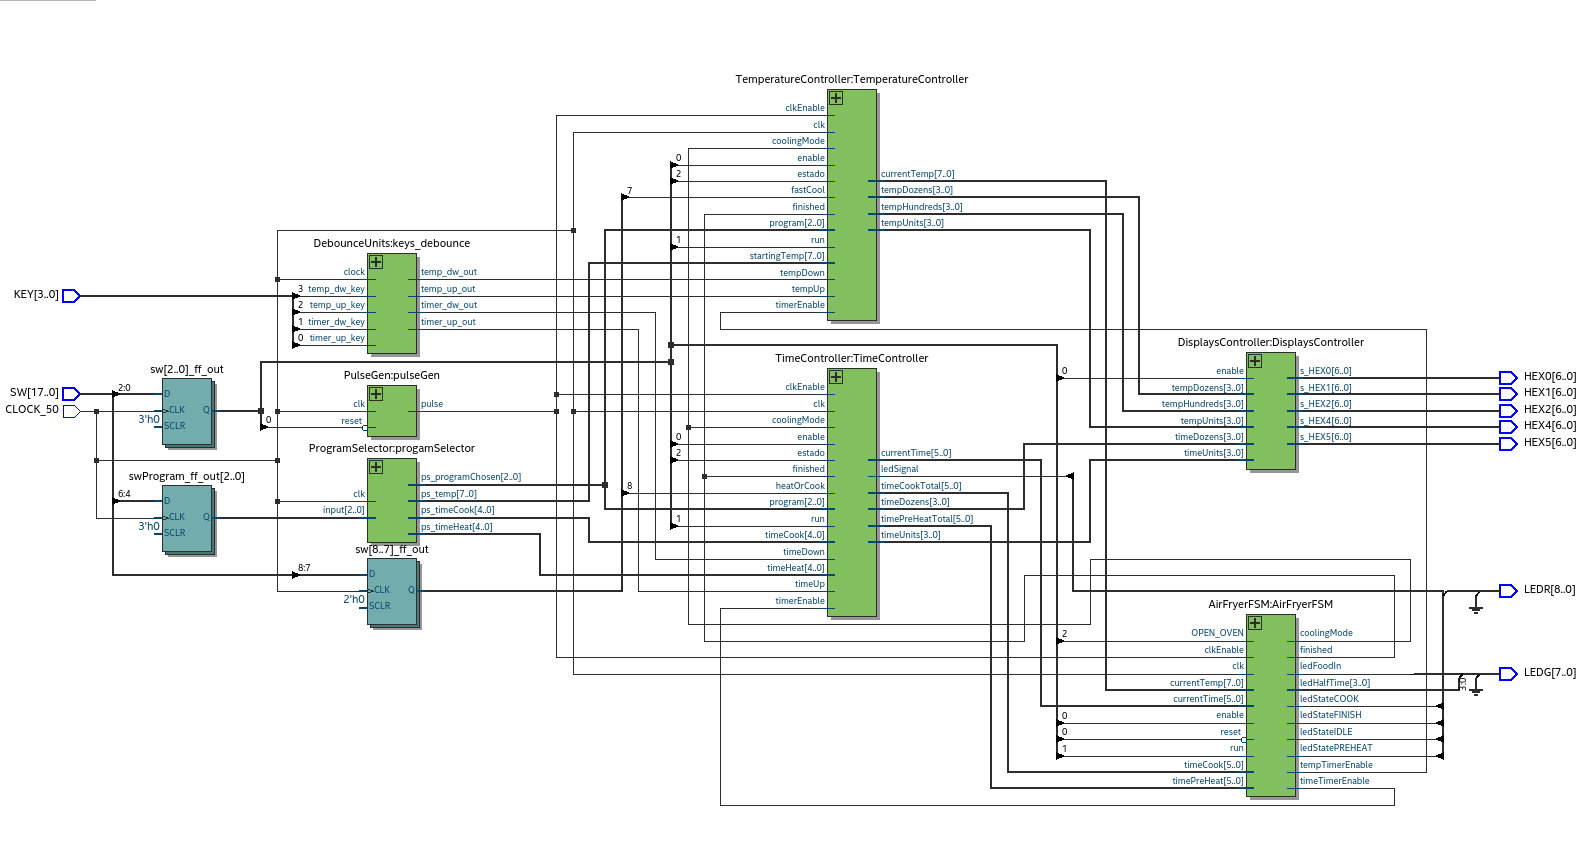
\includegraphics[width=\textwidth]{images/TopLevel.png}
    \caption{Representação do \textit{Top Level} do projeto}
    \label{fig:toplevel}
\end{figure}

\begin{itemize}
    \item \textbf{Debounce Unit} - Componente responsável pelo controlo das \textit{KEYs}. A sua utilização é essencial para eliminar o ruído elétrico (\textit{bounce}) gerado por interruptores mecânicos. Este componente pode ser modulado de forma a garantir que apenas um sinal limpo e estável seja enviado.
    \item \textbf{Pulse Generator} - Produz sinais elétricos periódicos com uma frequência ajustável, também conhecidos como pulsos. O sinal produzido foi utilizado no \textit{Timer} presente em cada um dos controladores (tempo e temperatura) para gerar um sinal com frequência de 1 \textit{Hertz}.
    \item \textbf{Program Selector} - Utilizado para gerir os tempos e temperaturas definidos por cada um dos programas existentes.
    \item \textbf{Temperature Controller} -  Bloco complexo responsável pelo controlo da temperatura durante os diferentes estados de operação do AirFryer. Responsável também pela edição da temperatura no modo \textit{USER}. Este bloco instância um \textit{Timer} e um \textit{Counter} para gerir a contagem e a variação da temperatura.
        \begin{itemize}
            \item \textbf{Timer} - Utilizado de forma a gerar um sinal periódico baseado no sinal de habilitação fornecido pelo gerador de pulsos e na frequência do sinal de relógio. É utilizado para sincronizar a atualização da temperatura.
            \item \textbf{Counter} - Utilizado para incrementar ou decrementar a temperatura com base no estado atual do sistema (Aquecimento ou Arrefecimento). Ajusta a temperatura com \textit{STEPs} definidos, garantido também que a temperatura permanece dentro dos limites establecidos.
        \end{itemize}
    \item \textbf{Time Controller} - Responsável por gerir os tempos de pré-aquecimento e cocção, além de permitir a edição desses tempos no modo \textit{USER}. Este bloco também instancia um \textit{Timer}.
    \item \textbf{Display Controller} - Responsável por converter binários da temperatura e tempo em sinais adequados para serem exibidos em displays de sete segmentos. Utiliza \textit{Decoders}
        \begin{itemize}
            \item \textbf{Decoder} - Converte valores binários de 4 bits (representado dígitos de 0 a 9) em sinais que controlam displays de 7 segmentos. É utilizado para exibir unidade, dezenas e centenas de valores de temperatura e tempo.
        \end{itemize}
    \item \textbf{AirFryer FSM} - Responsável por controlar os diferentes estados operacionais do AirFryer, incluindo os estados de espera, pré-aquecimento, cocção, finalização e arrefecimento. Garante que o sistema transita corretamente entre esses estados com base nas entradas e condições atuais.
\end{itemize}


%%%%%%%%%%%%%%%%%%%%%%%%%%%%%%%% Implementação %%%%%%%%%%%%%%%%%%%%%%%%%%%%%%%%
\chapter{Implementação}
\label{chap.arquitetura}
Este projeto está amplamente focado numa máquina de estados finitos, mais especificamente, numa máquina de Mealy, que depende tanto de seu estado atual quanto das suas entradas. Na Figura \ref{fig:fsm}, é possível visualizar o diagrama de estados da máquina. Abaixo, são descritos cada um dos seus estados: \\

\begin{figure}[H]
    \centering
    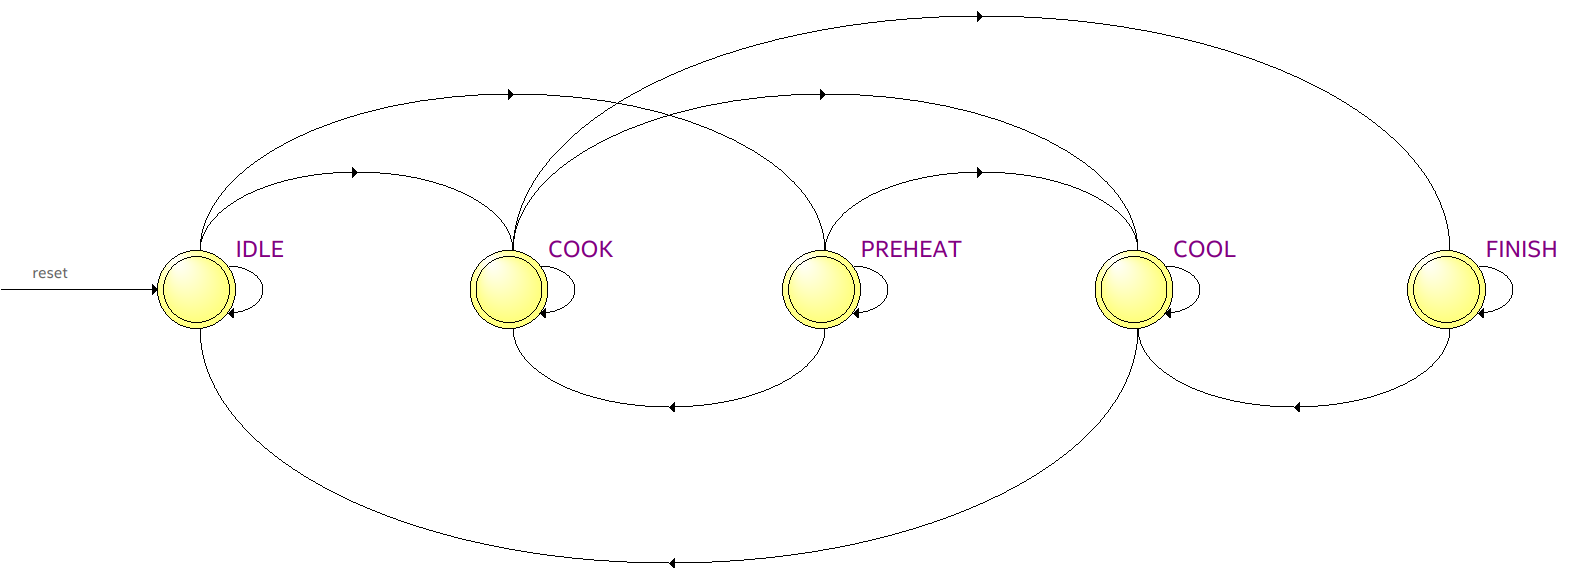
\includegraphics[width=\textwidth]{images/FSM.png}
    \caption{Representação da Máquina De Estados}
    \label{fig:fsm}
\end{figure}

\begin{itemize}
    \item \textbf{IDLE} - Estado inicial da máquina. Permite ao usuário selecionar o programa desejado, ajustar o tempo de cocção e pré-aquecimento, e definir a temperatura. O LED de "foodIn" acende se o programa não requer pré-aquecimento, indicando que a comida deve ser colocada imediatamente.
    
    \item \textbf{COOK} - Estado de cocção. A comida é cozida conforme os parâmetros definidos. O LED de cocção acende. Quando metade do tempo de cocção é atingido, os LEDs de \textit{HalfTime} piscam com uma frequência de 2 \textit{Hertz}. A transição para o estado FINISH ocorre quando o tempo de cocção acaba.

    \item \textbf{PREHEAT} - Estado de pré-aquecimento. A máquina aquece até à temperatura desejada antes de iniciar a cocção. Quando o tempo de pré-aquecimento termina, o LED de foodIn acende para indicar que a comida deve ser colocada. O LED de pré-aquecimento acende. 

    \item \textbf{FINISH} - Indica que o processo de cocção está concluído. Os LEDs de \textit{HalfTime} permanecem acesos. A máquina aguarda o usuário retirar a comida antes de entrar em modo de arrefecimento.

    \item \textbf{COOL} - Estado de arrefecimento. A máquina arrefece até a uma temperatura segura. Quando a temperatura interna atinge os 20ºC e a cuba está fechada, a máquina retorna ao estado \textit{IDLE}.
\end{itemize}

%%%%%%%%%%%%%%%%%%%%%%%%%%%%%%%% Manual do Utilizador %%%%%%%%%%%%%%%%%%%%%%%%%%%%%%%%
\chapter{Manual do Utilizador}
\label{chap.manualUtilizador}
\section{Programas}

\begin{table}[H]
\centering
\begin{tabular}{|c|c|c|c|c|}
\hline
\textbf{Programa} & \textbf{Switch} & \textbf{Temperatura} & \textbf{Tempo Pré-aquecimento} & \textbf{Tempo Cocção} \\ \hline
\textbf{Default}           & 000 & 200°    & N/A       & 18 mins    \\ \hline
\textbf{User}              & 001 & Usuário & Usuário   & Usuário    \\ \hline
\textbf{Rissóis}           & 010 & 180°    & 3 mins    & 15 mins    \\ \hline
\textbf{Batatas}           & 011 & 200°    & 5 mins    & 20 mins    \\ \hline
\textbf{Filetes de peixe}  & 100 & 170°    & 3 mins    & 20 mins    \\ \hline
\textbf{Hambúrguer}        & 101 & 170°    & 5 mins    & 20 mins    \\ \hline
\end{tabular}
\caption{Programas da AirFryer}
\label{tab:programas}
\end{table}
\par

A secção \textbf{Switch} refere-se à sequência de interruptores "Programas" \ (Ver figura \ref{fig:fpga}) que devem estar ligados (da direita para a esquerda) para alcançar cada um dos programas.

\section{Modo de utilização}
Ao ligar a máquina, esta inicia no modo \textit{IDLE}. O programa padrão selecionado ao ligar a máquina é o programa \textit{Default}. Usando os \textit{switches} disponíveis, o utilizador pode selecionar um dos programas disponíveis, conforme detalhado na Tabela \ref{tab:programas}.

Se o utilizador optar pelo modo \textit{USER}, terá a capacidade de personalizar os seguintes parâmetros:
\begin{itemize}
    \item \textbf{Temperatura}: O utilizador pode definir a temperatura desejada para a cocção.
    \item \textbf{Tempo de Pré-aquecimento}: O tempo necessário para pré-aquecer a máquina antes de iniciar a cocção, durante o qual a cuba de cocção deve estar vazia. \footnote{Durante a personalização dos tempos, é necessário acionar o interruptor "Tempo Cocção ou Pré-Aquecimento"\ para fazer a edição do tempo de pré-aquecimento}
    \item \textbf{Tempo de Cocção}: O tempo total de cocção dos alimentos após o pré-aquecimento.
\end{itemize}
  

Após a seleção do programa desejado e o início do funcionamento da AirFryer, se o programa incluir tempo de pré-aquecimento, a máquina começará a aquecer até atingir a temperatura alvo. Quando o pré-aquecimento terminar, a máquina sinalizará a necessidade de inserção dos alimentos. Após a inserção dos mesmos, a máquina entra no estado de cocção, onde inicia o processo de cozinhar. A qualquer momento durante a cocção, é possível abrir a cuba para rodar ou agitar os alimentos.
\par
Ao final do processo de cocção, ao desligar o modo RUN e abrir a cuba, a máquina começará a arrefecer naturalmente. Se o usuário desejar, pode ainda ativar o modo de arrefecimento rápido acionando o interruptor de arrefecimento.

\section{Esquema da máquina}
\begin{figure}[H]
    \centering
    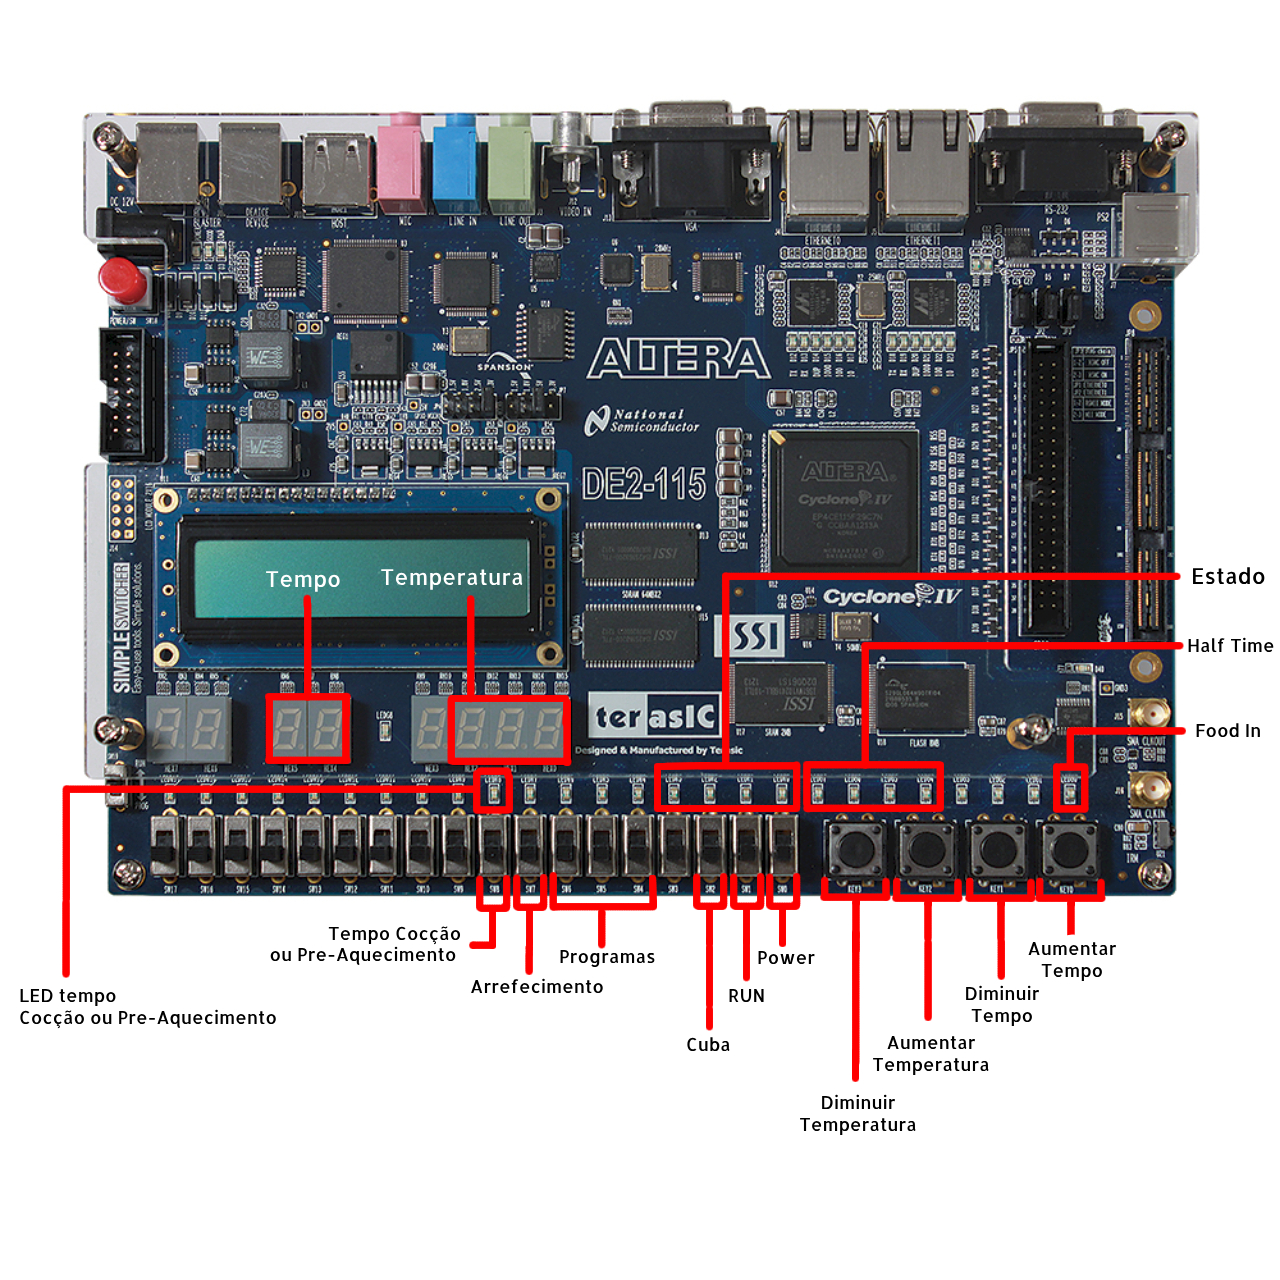
\includegraphics[width=\textwidth]{images/FPGA_Ilustrada.jpg}
    \caption{Ilustração do Esquema da máquina}
    \label{fig:fpga}
\end{figure}


%%%%%%%%%%%%%%%%%%%%%%%%%%%%%%%% Conclusões e Contribuições %%%%%%%%%%%%%%%%%%%%%%%%%%%%%%%%
\chapter{Conclusão}
\section{Conclusões}
O desenvolvimento deste projeto final proporcionou uma valiosa oportunidade de aplicar na prática os conhecimentos adquiridos ao longo da cadeira de \ac{lsd}. Através da implementação de uma AirFryer controlada digitalmente, foi possível explorar diversas áreas, incluindo a programação em \ac{vhdl} e o  seu uso com FPGAs.

Este projeto não só cumpriu os seus objetivos principais, como também proporcionou um aprofundamento significativo no conhecimento dos sistemas em questão, mas também do design de hardware digital. 

Em suma, o projeto da AirFryer controlada digitalmente mostrou-se uma experiência enriquecedora, destacando a importância da integração entre teoria e prática no campo da engenharia eletrónica. 

\section{Validação}
Ao longo do nosso projeto, enfrentámos diversas advertências relacionadas à simulação e validação. Por isso, a principal forma de validarmos os resultados foi através de testes práticos na placa. Como o trabalho foi desenvolvido com base em intervalos de tempo muito longos, em segundos, tornou-se difícil e inconveniente utilizar tanto o simulador quanto a \textit{testbench}.

\section{Contribuições dos autores}
Cada autor contribuiu igualmente para o produto final do trabalho, sendo justamente atribuído a nota de 50\% a cada um.

%%%%%%%%%%%%%%%%%%%%%%%%%%%%%%%%%
\chapter*{Acrónimos}
\begin{acronym}
\acro{ua}[UA]{Universidade de Aveiro}
\acro{leci}[LECI]{Licenciatura em Engenharia de Computadores e Informática}
\acro{lsd}[LSD]{Laboratório de Sistemas Digitais}
\acro{vhdl}[VHDL]{VHSIC Hardware Description Language}
\end{acronym}
%%%%%%%%%%%%%%%%%%%%%%%%%%%%%%%%%

\begin{flushright}
    \today
\end{flushright}

\end{document}